\documentclass[oneside]{book}

% -> Pacotes usados em main.tex
\usepackage[brazil]{babel}
\usepackage[utf8]{inputenc}
\usepackage{graphicx}

% -> Pacotes usados em cvalice.tex
\usepackage{titlesec}

% ->B: Pacotes usados em cvbreno2.tex
\usepackage[most]{tcolorbox}
\usepackage[a4paper, top=0.1cm, bottom=0.1cm, left=0.1cm, right=0.1cm]{geometry}

% -> Pacotes usados em cvgustavo.tex
\usepackage{color}
\usepackage{setspace}
\usepackage{sectsty}

% ->Pacotes usados em cleomarTex.tex
\usepackage{subfigure}
\usepackage{xstring, xifthen}
\usepackage{enumitem}
\usepackage{changepage}
\usepackage{fontawesome}
\usepackage{paracol}
\usepackage{tikzpagenodes}
\usetikzlibrary{calc}
\usepackage{lmodern}
\usepackage{atbegshi}
\usepackage{fancyhdr}
\usepackage{array}
\usepackage{tikz}			
\usepackage{ragged2e}	
\usetikzlibrary{shapes, backgrounds,mindmap, trees}
\usepackage{transparent}
\usepackage[hidelinks]{hyperref}

% -> Pacotes usados em joaomendes.tex
%adicionados agora, vou deixar separado só p ficar mais de fácil acesso
\usepackage{fontawesome}
\usepackage{paracol}
\usepackage{tikzpagenodes}
\usetikzlibrary{calc}
\usepackage{lmodern}
%\usepackage{multicol}
\usepackage{atbegshi}
\usepackage[a4paper]{geometry}
\usepackage{fancyhdr}
\usepackage{array}
\usepackage{graphicx}
%\usepackage{wrapfig}
\usepackage{float}
\usepackage{tikz}	
\usepackage{ragged2e}	
\usepackage{transparent}
\usepackage{color}

% -> Pacotes usados em cvequipe.tex
\usepackage{xltabular}
\usepackage{multicol}
\usepackage{indentfirst}
\usepackage{float}

% -> Pacotes usados em referencias.bib
\usepackage[nottoc]{tocbibind} 

% ->B: AVISO: A gambiarra a seguir pode te matar.
\title{
	\begin{figure}[h]
		\centering
		
\includegraphics[width=10cm]{imagens/logo.png} 		
	\end{figure}
	\textbf{Trabalho de Introdução à Computação}}
\author{
	Alice Pereira de Aguilar Penido \thanks{alicepenido1@gmail.com} \\
	Breno Marques Azevedo \thanks{eborn.azevedo@gmail.com} \\
	Cleomar Felipe Rabelo Antoszczyszyn \thanks{cleomarfelipe@gmail.com} \\
	Gustavo Ramalho \thanks{gustavoramalho384@gmail.com} \\
	João Victor Mendes  \thanks{j.victor8@hotmail.com}
}
\date{\today} % -> Iniciado em 07/03/2020

\pagenumbering{Roman}
\begin{document}
	% ->B: Selecionei a fonte Computer Modern Roman, pois ela está mais de acordo com o modelo de trabalhos científicos(eu acho).
	{\fontfamily{cmr}\selectfont 
		\maketitle
		\newgeometry{left=1cm, right=1cm, bottom=1cm, top=1cm}
		\thispagestyle{empty}
		\setcounter{page}{1}
		\tableofcontents
		\listoffigures
		
		\chapter{Alice Pereira de Aguilar Penido}
		\pagenumbering{arabic}
		\section*{Segue na próxima página o currículo de Alice Pereira de Aguilar Penido}
		\restoregeometry
		\input{alice/cvalice.tex}
		
		\newgeometry{left=1cm, right=1cm}
		\chapter{Breno Marques Azevedo}
		\section*{Segue na próxima página o currículo de Breno Marques Azevedo\cite{quantbytes}}
		\restoregeometry
		\newpage
		\input{breno/cvbreno2.tex}
	}
	
	\newgeometry{left=1cm, right=1cm}
	\chapter{Cleomar Felipe Rabelo Antoszczyszyn}
	\section*{O currículo de Cleomar Felipe Rabelo Antoszczyszyn encontra-se na próxima página}
	\restoregeometry
	\newpage
	\input{cleomar/cvcleomar.tex}
	% ->B: De novo a fonte Computer Modern Roman.
	{\fontfamily{cmr}\selectfont
		
		\chapter{Gustavo Ramalho}
		\section*{Segue na próxima página o currículo de Gustavo Ramalho}
		\newpage
		\input{gustavo/cvgustavo.tex}
		
		\chapter{João Victor Mendes}
		\section*{Segue na próxima página o currículo de João Victor Mendes}
		\newpage
		%Olá Tio Rafa! sou o aluno João Victor Mendes (211708033)

%informações e comentários extras inúteis caso o tio rafa esteja entediado:

%optei por usar um template ao invés de fazer do zero pois achei que seria uma experiência interessante aprender a mudar configurações como cor (lancei um azul FGV em todo lugar) e excluir/adicionar seções em um documento que não entendo o que cada coisa significa, e realmente, foi divertidíssimo, bati bastante a cabeça para mexer em algumas coisas, eu havia feito um currículo completo assim em outro documentclass e percebi só um tempão depois hahahah;

%como com certeza ainda não tenho conteúdo o suficiente para duas páginas de currículo, a segunda não ficou tão objetiva, mas acho que foram comentários úteis sobre diversos pontos do currículo que acabariam gerando dúvidas por si só, como a graduação na UTFPR sem ano de início;

%também optei por matar algumas fadas latino-americanas traduzindo o nome das graduações e cursos, fiquei em dúvida sobre o que seria mais correto, isso ou manter em português;

%pensei em editar a foto por conta de tudo aquilo sobre cabelo comprido e mercade de trabalho, talvez algo mais formal fosse melhor pra um currículo, porém não sei acho que eu não abriria mão da minha identidade pra trabalhar em um lugar :p resolvi manter



%-----------------------------------------------------------------------------------------------------------------------------------------------%
%	The MIT License (MIT)
%
%	Copyright (c) 2021 Philip Empl
%
%	Permission is hereby granted, free of charge, to any person obtaining a copy
%	of this software and associated documentation files (the "Software"), to deal
%	in the Software without restriction, including without limitation the rights
%	to use, copy, modify, merge, publish, distribute, sublicense, and/or sell
%	copies of the Software, and to permit persons to whom the Software is
%	furnished to do so, subject to the following conditions:
%	
%	THE SOFTWARE IS PROVIDED "AS IS", WITHOUT WARRANTY OF ANY KIND, EXPRESS OR
%	IMPLIED, INCLUDING BUT NOT LIMITED TO THE WARRANTIES OF MERCHANTABILITY,
%	FITNESS FOR A PARTICULAR PURPOSE AND NONINFRINGEMENT. IN NO EVENT SHALL THE
%	AUTHORS OR COPYRIGHT HOLDERS BE LIABLE FOR ANY CLAIM, DAMAGES OR OTHER
%	LIABILITY, WHETHER IN AN ACTION OF CONTRACT, TORT OR OTHERWISE, ARISING FROM,
%	OUT OF OR IN CONNECTION WITH THE SOFTWARE OR THE USE OR OTHER DEALINGS IN
%	THE SOFTWARE.
%	
%
%-----------------------------------------------------------------------------------------------------------------------------------------------%


%============================================================================%
%
%	DOCUMENT DEFINITION
%
%============================================================================%

%\documentclass[10pt,A4,english]{book}	


%----------------------------------------------------------------------------------------
%	ENCODING
%----------------------------------------------------------------------------------------

% we use utf8 since we want to build from any machine
%\usepackage[utf8]{inputenc}		
%\usepackage[USenglish]{isodate}
%\usepackage{fancyhdr}
%\usepackage[numbers]{natbib}

%----------------------------------------------------------------------------------------
%	LOGIC
%----------------------------------------------------------------------------------------

% provides \isempty test
%\usepackage{xstring, xifthen}
%\usepackage{enumitem}
%\usepackage[english]{babel}
%\usepackage{blindtext}
%\usepackage{pdfpages}
%\usepackage{changepage}
%\usepackage{setspace}
%----------------------------------------------------------------------------------------
%	FONT BASICS
%----------------------------------------------------------------------------------------

% some tex-live fonts - choose your own

%\usepackage[defaultsans]{droidsans}
%\usepackage[default]{comfortaa}
%\usepackage{cmbright}
%\usepackage[default]{raleway}
%\usepackage{fetamont}
%\usepackage[default]{gillius}
%\usepackage[light,math]{iwona}
%\usepackage[thin]{roboto} 

% set font default
\renewcommand*\familydefault{\sfdefault} 	
%\usepackage[T1]{fontenc}

% more font size definitions
%\usepackage{moresize}

%----------------------------------------------------------------------------------------
%	FONT AWESOME ICONS
%---------------------------------------------------------------------------------------- 

% include the fontawesome icon set
%\usepackage{fontawesome}

% use to vertically center content
% credits to: http://tex.stackexchange.com/questions/7219/how-to-vertically-center-two-images-next-to-each-other
\newcommand{\vcenteredinclude}[1]{\begingroup
	\setbox0=\hbox{\includegraphics{#1}}%
	\parbox{\wd0}{\box0}\endgroup}
\newcommand{\tab}[1]{\hspace{.2\textwidth}\rlap{#1}}
% use to vertically center content
% credits to: http://tex.stackexchange.com/questions/7219/how-to-vertically-center-two-images-next-to-each-other
\newcommand*{\vcenteredhbox}[1]{\begingroup
	\setbox0=\hbox{#1}\parbox{\wd0}{\box0}\endgroup}

% icon shortcut
\newcommand{\icon}[3] { 							
	\makebox(#2, #2){\textcolor{maincol}{\csname fa#1\endcsname}}
}	


% icon with text shortcut
\newcommand{\icontext}[4]{ 						
	\vcenteredhbox{\icon{#1}{#2}{#3}}  \hspace{2pt}  \parbox{0.9\mpwidth}{\textcolor{#4}{#3}}
}

% icon with website url
\newcommand{\iconhref}[5]{ 						
	\vcenteredhbox{\icon{#1}{#2}{#5}}  \hspace{2pt} \href{#4}{\textcolor{#5}{#3}}
}

% icon with email link
\newcommand{\iconemail}[5]{ 						
	\vcenteredhbox{\icon{#1}{#2}{#5}}  \hspace{2pt} \href{mailto:#4}{\textcolor{#5}{#3}}
}

%----------------------------------------------------------------------------------------
%	PAGE LAYOUT  DEFINITIONS
%----------------------------------------------------------------------------------------

% page outer frames (debug-only)
% \usepackage{showframe}		

% we use paracol to display breakable two columns
%\usepackage{paracol}
%\usepackage{tikzpagenodes}
%\usetikzlibrary{calc}
%\usepackage{lmodern}
%\usepackage{multicol}
%\usepackage{lipsum}
%\usepackage{atbegshi}
% define page styles using geometry
%\usepackage[a4paper]{geometry}

% remove all possible margins
%\geometry{top=1cm, bottom=1cm, left=1cm, right=1cm}

%\usepackage{fancyhdr}
\pagestyle{empty}

% space between header and content
% \setlength{\headheight}{0pt}

% indentation is zero
\setlength{\parindent}{0mm}

%----------------------------------------------------------------------------------------
%	TABLE /ARRAY DEFINITIONS
%---------------------------------------------------------------------------------------- 

% extended aligning of tabular cells
%\usepackage{array}

% custom column right-align with fixed width
% use like p{size} but via x{size}
%\newcolumntype{x}[1]{%
%>{\raggedleft\hspace{0pt}}p{#1}}%


%----------------------------------------------------------------------------------------
%	GRAPHICS DEFINITIONS
%---------------------------------------------------------------------------------------- 

%for header image
%\usepackage{graphicx}

% use this for floating figures
% \usepackage{wrapfig}
% \usepackage{float}
% \floatstyle{boxed} 
% \restylefloat{figure}

%for drawing graphics		
%\usepackage{tikz}			
%\usepackage{ragged2e}	
\usetikzlibrary{shapes, backgrounds,mindmap, trees}

%----------------------------------------------------------------------------------------
%	Color DEFINITIONS
%---------------------------------------------------------------------------------------- 
%\usepackage{transparent}
%\usepackage{color}

% primary color
\definecolor{maincol}{RGB}{26, 44, 97}

% accent color, secondary
% \definecolor{accentcol}{RGB}{ 250, 150, 10 }

% dark color
\definecolor{darkcol}{RGB}{26, 44, 97}

% light color
\definecolor{lightcol}{RGB}{200,200,200}

\definecolor{accentcol}{RGB}{26, 44, 97}



% Package for links, must be the last package used
%\usepackage[hidelinks]{hyperref}

% returns minipage width minus two times \fboxsep
% to keep padding included in width calculations
% can also be used for other boxes / environments
\newcommand{\mpwidth}{\linewidth-\fboxsep-\fboxsep}



%============================================================================%
%
%	CV COMMANDS
%
%============================================================================%

%----------------------------------------------------------------------------------------
%	 CV LIST
%----------------------------------------------------------------------------------------

% renders a standard latex list but abstracts away the environment definition (begin/end)
\newcommand{\cvlist}[1] {
	\begin{itemize}{#1}\end{itemize}
}

%----------------------------------------------------------------------------------------
%	 CV TEXT
%----------------------------------------------------------------------------------------

% base class to wrap any text based stuff here. Renders like a paragraph.
% Allows complex commands to be passed, too.
% param 1: *any
\newcommand{\cvtext}[1] {
	\begin{tabular*}{1\mpwidth}{p{0.98\mpwidth}}
		\parbox{1\mpwidth}{#1}
	\end{tabular*}
}
\newcommand{\cvtextsmall}[1] {
	\begin{tabular*}{0.8\mpwidth}{p{0.8\mpwidth}}
		\parbox{0.8\mpwidth}{#1}
	\end{tabular*}
}
%----------------------------------------------------------------------------------------
%	CV SECTION
%----------------------------------------------------------------------------------------

% Renders a a CV section headline with a nice underline in main color.
% param 1: section title
\newcommand{\cvsection}[1] {
	\vspace{4pt}
	\cvtext{
		\textbf{\LARGE{\textcolor{darkcol}{#1}}}\\[-4pt]
		\textcolor{accentcol}{ \rule{0.2\textwidth}{0.5pt} } \\
	}
}

\newcommand{\cvsectionsmall}[1] {
	\vspace{4pt}
	\cvtext{
		\textbf{\Large{\textcolor{darkcol}{#1}}}\\[-4pt]
		\textcolor{accentcol}{ \rule{0.2\textwidth}{0.5pt} } \\
	}
}

\newcommand{\cvheadline}[1] {
	\vspace{6pt}
	\cvtext{
		\textbf{\Huge{\textcolor{accentcol}{#1}}}\\[-4pt]
		
	}
}

\newcommand{\cvsubheadline}[1] {
	\vspace{6pt}
	\cvtext{
		\textbf{\huge{\textcolor{darkcol}{#1}}}\\[-4pt]
		
	}
}
%----------------------------------------------------------------------------------------
%	META SKILL
%----------------------------------------------------------------------------------------

% Renders a progress-bar to indicate a certain skill in percent.
% param 1: name of the skill / tech / etc.
% param 2: level (for example in years)
% param 3: percent, values range from 0 to 1
\newcommand{\cvskill}[3] {
	\begin{tabular*}{1\mpwidth}{p{0.72\mpwidth}  r}
		\textcolor{black}{\textbf{#1}} & \textcolor{maincol}{#2}\\
	\end{tabular*}%
	
	\hspace{4pt}
	\begin{tikzpicture}[scale=1,rounded corners=2pt,very thin]
		\fill [lightcol] (0,0) rectangle (1\mpwidth, 0.15);
		\fill [accentcol] (0,0) rectangle (#3\mpwidth, 0.15);
	\end{tikzpicture}%
}


%----------------------------------------------------------------------------------------
%	 CV EVENT
%----------------------------------------------------------------------------------------

% Renders a table and a paragraph (cvtext) wrapped in a parbox (to ensure minimum content
% is glued together when a pagebreak appears).
% Additional Information can be passed in text or list form (or other environments).
% the work you did
% param 1: time-frame i.e. Sep 14 - Jan 15 etc.
% param 2:	 event name (job position etc.)
% param 3: Customer, Employer, Industry
% param 4: Short description
% param 5: work done (optional)
% param 6: technologies include (optional)
% param 7: achievements (optional)
\newcommand{\cvevent}[7] {
	
	% we wrap this part in a parbox, so title and description are not separated on a pagebreak
	% if you need more control on page breaks, remove the parbox
	\parbox{\mpwidth}{
		\begin{tabular*}{1\mpwidth}{p{0.66\mpwidth}  r}
			\textcolor{black}{\textbf{#2}} & \colorbox{accentcol}{\makebox[0.32\mpwidth]{\textcolor{white}{\textbf{#1}}}} \\
			\textcolor{maincol}{#3} & \\
		\end{tabular*}\\[8pt]
		
		\ifthenelse{\isempty{#4}}{}{
			\cvtext{#4}\\
		}
	}
	\vspace{4pt}
}


%----------------------------------------------------------------------------------------
%	 CV META EVENT
%----------------------------------------------------------------------------------------

% Renders a CV event on the sidebar
% param 1: title
% param 2: subtitle (optional)
% param 3: customer, employer, etc,. (optional)
% param 4: info text (optional)
\newcommand{\cvmetaevent}[4] {
	\textcolor{maincol} { \cvtext{\textbf{\begin{flushleft}#1\end{flushleft}}}}
	
	\ifthenelse{\isempty{#2}}{}{
		\textcolor{black} {\cvtext{\textbf{#2}} }
	}
	
	\ifthenelse{\isempty{#3}}{}{
		\cvtext{{ \textcolor{maincol} {#3} }}\\
	}
	
	\cvtext{#4}\\[14pt]
}

%---------------------------------------------------------------------------------------
%	QR CODE
%----------------------------------------------------------------------------------------

% Renders a qrcode image (centered, relative to the parentwidth)
% param 1: percent width, from 0 to 1
\newcommand{\cvqrcode}[1] {
	\begin{center}
		\includegraphics[width={#1}\mpwidth]{qrcode}
	\end{center}
}


% HEADER AND FOOOTER 
%====================================
\newcommand\Header[1]{%
	\begin{tikzpicture}[remember picture,overlay]
		\fill[accentcol]
		(current page.north west) -- (current page.north east) --
		([yshift=50pt]current page.north east|-current page text area.north east) --
		([yshift=50pt,xshift=-3cm]current page.north|-current page text area.north) --
		([yshift=10pt,xshift=-5cm]current page.north|-current page text area.north) --
		([yshift=10pt]current page.north west|-current page text area.north west) -- cycle;
		\node[font=\sffamily\bfseries\color{white},anchor=west,
		xshift=0.7cm,yshift=-0.32cm] at (current page.north west)
		{\fontsize{12}{12}\selectfont {#1}};
	\end{tikzpicture}%
}

\newcommand\Footer[1]{%
	\begin{tikzpicture}[remember picture,overlay]
		\fill[lightcol]
		(current page.south east) -- (current page.south west) --
		([yshift=-80pt]current page.south east|-current page text area.south east) --
		([yshift=-80pt,xshift=-6cm]current page.south|-current page text area.south) --
		([xshift=-2.5cm,yshift=-10pt]current page.south|-current page text area.south) --	
		([yshift=-10pt]current page.south east|-current page text area.south east) -- cycle;
		\node[yshift=0.32cm,xshift=9cm] at (current page.south) {\fontsize{10}{10}\selectfont \textbf{\thepage}};
	\end{tikzpicture}%
}


%=====================================
%============================================================================%
%
%
%
%	DOCUMENT CONTENT
%
%
%
%============================================================================%
%\begin{document}

\columnratio{0.31}
\setlength{\columnsep}{2.2em}
%\setlength{\columnseprule}{4pt}
\colseprulecolor{white}


% LEBENSLAUF HIERE
%\AtBeginShipoutFirst{\Header{CV}\Footer{1}}
%\AtBeginShipout{\AtBeginShipoutAddToBox{\Header{CV}\Footer{2}}}

\newpage

\colseprulecolor{lightcol}
\columnratio{0.31}
\setlength{\columnsep}{2.2em}
%\setlength{\columnseprule}{4pt}
\begin{paracol}{2}
	
	
	\begin{leftcolumn}
		%---------------------------------------------------------------------------------------
		%	META IMAGE
		%----------------------------------------------------------------------------------------
		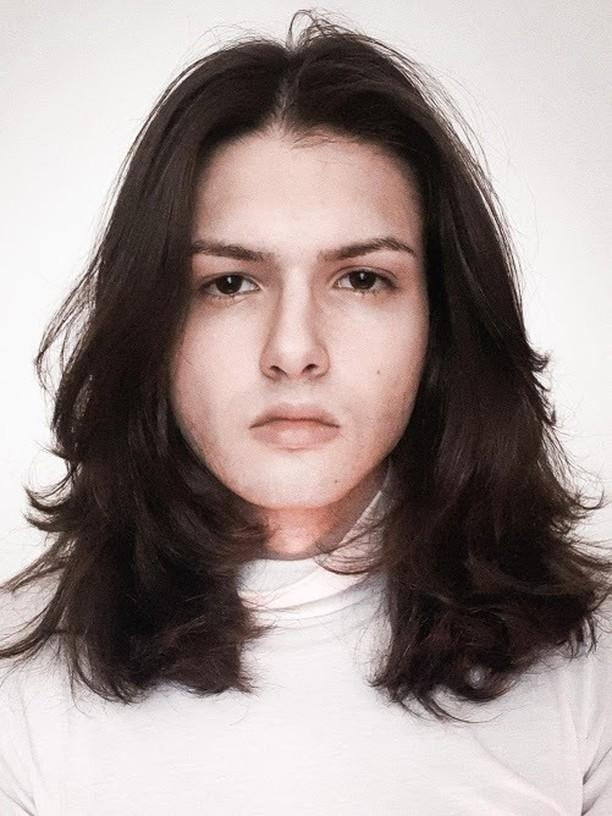
\includegraphics[width=\linewidth]{victormendes/picjoao.jpg}	%trimming relative to image size
		
		
		%---------------------------------------------------------------------------------------
		%	META SKILLS
		%----------------------------------------------------------------------------------------
		\fcolorbox{white}{white}{\begin{minipage}[c][1.5cm][c]{1\mpwidth}
				\Large{\textbf{\textcolor{maincol}{João Victor Mendes}}} \\[1pt]
				\normalsize{ \textcolor{maincol} {Aspiring Data Scientist} }
		\end{minipage}} \\\setstretch{0.9}
		\icontext{CaretRight}{12}{15/07/2002}{black}\\[6pt]
		\icontext{CaretRight}{12}{+55 42 9 9806-1534}{black}\\[6pt]
		\icontext{CaretRight}{12}{j.victor8@hotmail.com}{black}\\[6pt]
		
		\cvsection{Biography}
		\vspace{4pt}
		\setstretch{0.9}
		\cvtext{I am a curious born, I always liked to learn about everything and understand how information connects and how it influences everything in the world. Seeing the world with a careful data bias has always been beyond a hobby, a way of life and a philosophy for me.}
		
		
		\setstretch{0.9}
		\cvsection{Skills}
		
		\cvskill{Conflict Resolution} {} {0.83} \\[-2pt]
		
		\cvskill{Leadership} {} {0.68} \\[-2pt]
		
		\cvskill{Communication} {} {0.79} \\[-2pt]
		
		\cvskill{Aministrative} {} {0.72} \\[-2pt]
		
		\cvskill{Time Management} {} {0.52} \\[-2pt]
		
		\cvskill{Portuguese} {L1} {1} \\[-2pt]
		
		\cvskill{English} {B1} {0.65} \\[-2pt]
		\vfill\null
		\vfill\null
		
		
		\newpage
		%---------------------------------------------------------------------------------------
		%	EDUCATION
		%----------------------------------------------------------------------------------------
		\vspace{0.5pt}
		\cvsection{Awards}
		\vspace{0.5pt}
		
		\setstretch{0.5}
		\large
		\cvevent
		{2018}{First Place \newline \newline SENAI's \newline Inovation Grand Pix.}
		\vfill\null
		\vfill\null
		
		\cvevent
		{2016}{Silver Medal \newline \newline OBMEP.}
		\vfill\null
		\vfill\null
		
		\cvevent
		{2015}{Honorabel\newline Mention \newline \newline OBMEP.}
		\vfill\null
		\vfill\null
		
		\cvevent
		{2014}{Bronze Medal \newline \newline OBMEP.}
		\vfill\null
		\vfill\null
		
		\cvevent
		{2013}{Honorabel \newline Mention  \newline \newline OBMEP.}
		\vfill\null
		\vfill\null
		
		
		
		
		%
		%\cvsection{Projekte}
		
		%	\cvlist{
		%		\item \hyperlink{https://github.com/philipempl/ether-twin}{\textbf{Ether-Twin.}}\\ Ethereum Applikation für Digital Twins.
		%		\item \hyperlink{https://github.com/philipempl/Peter-Pan}{\textbf{Peter Pan.}}\\ Koch-App (t.b.a.).
		%		\item \hyperlink{https://github.com/philipempl/Innovation-Tool}{\textbf{Innovation Tool.}}\\ Webcrawler für \hyperlink{https://ibi.de/}{Ibi}.
		%		\item \hyperlink{https://github.com/philipempl/cozone}{\textbf{COZONE.}} \\ Soziales Netzwerk (t.b.a.).
		%		\item \hyperlink{https://github.com/geritwagner/enlit}{\textbf{ENLIT.}}\\ Exploring new Literature (Bachelorarbeit).
		%		\item \textbf{Crowdfunding.} \\Modul mit \hyperlink{https://senacor.com/}{Senacor} für \hyperlink{https://www.paydirekt.de/}{paydirekt}.
		%		}
		
		
		
		%\cvqrcode{0.3}
		
	\end{leftcolumn}
	\begin{rightcolumn}
		%---------------------------------------------------------------------------------------
		%	TITLE  HEADER
		%----------------------------------------------------------------------------------------
		
		
		%---------------------------------------------------------------------------------------
		%	PROFILE
		%----------------------------------------------------------------------------------------
		
		
		\cvsection{Interests}
		\vspace{3pt}
		
		\cvtext{Help the company to optimize the Finance and Marketing processes to generate better results.}
		
		%---------------------------------------------------------------------------------------
		%	WORK EXPERIENCE
		%----------------------------------------------------------------------------------------
		
		\vspace{0.9pt}
		\cvsection{Education}
		\vspace{0.9pt}
		
		{\setstretch{0.9}
			\cvevent
			{2021 - Today}
			{Graduation in Data Sciente}
			{FGV EMAp \newline Rio de Janeiro, Brasil}
			\vfill\null
			\vfill\null
			
			\cvevent
			{-}
			{Graduation in Computer Information Systems}
			{UTFPR \newline Curitiba, Brasil}
			\vfill\null
			\vfill\null
			
			\cvevent
			{2020 - 2020}
			{Discontinued - Graduation in Economics}
			{FGV EPGE \newline Rio de Janeiro, Brasil}
			\vfill\null
			\vfill\null
			
			\cvevent
			{2018 - 2019}{Technical Course in Administrative Assistant}{SENAI/PR \newline União da Vitória, Brasil.}
			\vfill\null
			\vfill\null
			
			\cvevent
			{2017 - 2019}{Secondary Education}{SESI/PR \newline União da Vitória, Brasil.}
			\vfill\null
			\vfill\null
			
			\cvevent
			{2015-2015}{Discontinued - Jr. Scientific Initiation}{PIC-OBMEP \newline União da Vitória, Brasil.}
			\vfill\null
			\vfill\null
			
			\cvevent
			{2014-2014}{Jr. Scientific Initiation}{PIC-OBMEP \newline União da Vitória, Brasil.}
			\vfill\null
			\vfill\null
			
			\cvevent
			{2007-2016}{Elementary Education}{CENM \newline Bituruna, Brasil.}
			\vfill\null
			\vfill\null}
		
		\cvsection{Experience}
		
		{\setstretch{0.6}
			\cvevent
			{2019-2019}{Young Apprentice}{SESI/PR \newline União da Vitória, Brasil.}
			\vfill\null	
			\vfill\null}
		
		\newpage
		
		\cvsection{Other Experiences/Education}
		
		\setstretch{0.6}
		
		\cvevent
		{2018-2018} {"Introduction to the Business World" Program} {Junior Achievement \newline União da Vitória, Brasil.}
		\vfill\null
		\vfill\null
		
		\cvevent
		{2018-2018} {"Let’s Talk Ethics" Program} {Junior Achievement \newline União da Vitória, Brasil.}
		\vfill\null
		\vfill\null
		
		\cvevent
		{2018-2018} {"Mini Company" Program} {Junior Achievement \newline União da Vitória, Brasil.}
		\vfill\null
		\vfill\null
		
		\cvevent
		{2018-2018} {"Personal Savings" Program} {Junior Achievement \newline União da Vitória, Brasil.}
		\vfill\null
		\vfill\null
		
		\small
		\cvsection{Extra-Information}
		
		
		\subsection*{Education: Extra-Information}
		I got to start 4 Jr. scientific initiations by OBMEP but I completed only one due to a problem involving lack of access to the internet and devices such as notebook and cell phone (the Scientific Initiations were entirely online);\newline
		
		I started my undergraduate degree in Economics as a scholarship holder at CDMC,because I always wanted to understand how the world worked and why things happened and saw a way for this understanding through economics;\newline
		
		However, over time, I discovered that I would have much more opportunities to study what I like in Data Science, so I decided to change my degree;\newline
		
		I have been pre-enrolled at UTFPR since the middle of 2020, but because of the pandemic I have no news of when classes will start;\newline
		
		
		\subsection*{Awards: Extra-Information}
		
		I also won prizes in other minor competitions involving creativity in the most diverse ways, from making furniture to cooking (at SESI and SENAI);\newline
		
		I won Silver Medal in a municipal writing competition, and won some other regional prizes in Chess and Judo .\newline
		
		
		\subsection*{Experience: Extra-Information}
		
		I had other experiences related to the labor market other than formal jobs:\newline
		
		High school at SESI is a great teamwork experience within a company; there I was also Vice President of the student union.\newline
		
		In Junior Achievment’s "Mini Company" Program, we created and managed a company during the period of one year, our company (which I was President) ranked third in the region and among the top 10 in the state;\newline
		
		
		\subsection*{Languages: Extra-Information}
		
		My native language is Brazilian Portuguese, because of this I naturally understand Spanish in a basic way;\newline
		
		I didn’t have a good formal English teaching until the end of high school, but I learned alone enough to be leveled in book 5 of BRASAS and book 7 of CCAA, now I am studying book 6 of BRASAS and I plan to continue until the conclusion of the book 10;\newline
		
		I intend to study French to try to exchange in France through FGV;
		
		
		
		
	\end{rightcolumn}
\end{paracol}

%\end{document}
		
		\chapter{Equipe}
		\section*{Segue na próxima página o currículo da equipe profissional de League of Legends\cite{prabhu}}
		\newpage
		% Créditos
%AuthorOmkar            Prabhu
%LicenseCreative        Commons CC BY 4.0
%Abstract               Very Simple LaTeX Resume Template
%Link                   https://pt.overleaf.com/latex/templates/resume-template/gxymbfbhdjwk
% ------------------------------------------------------------------------

\begin{tabularx}{\linewidth}{@{}m{0.8\textwidth} m{0.2\textwidth}@{}}
	\Large{Equipe Trabson 2} &  \\
	\small{contatrabson@gmail.com} & \\
	Rio de Janeiro - Brasil
\end{tabularx}

\textcolor{mygray}{\rule{\textwidth}{1pt}}

\section*{Finalidade}
Este currículo está sendo apresentado para todas as empresas de dentro e fora do e-sports de League of Legends\cite{khawli} que possuem interesse em investir na equipe de LoL Trabson 2 - a T2. A T2 foi campeã de tudo que disputou no ano de 2020 e procura recursos para construir a nova Gaming House e conceder um treinamento mais de ponta para os players. Preços serão negociados com investidores via inbox.

\section*{Premiações da Equipe}
\begin{itemize}
	\item 1 Mundial de League of Legends 2020 - (1 participação)
	\item 1 Mid Season Invitational - 2020 (1 participação)
	\item 1 League of Legends European Championship - 2020.1, 2020.2 (2 participações)
	\item 1 Torneio de Férias - Summer 2020 (1 participação)
\end{itemize}
\newpage

\begin{tabularx}{\linewidth}{@{}m{0.8\textwidth} m{0.2\textwidth}@{}}
	\large{Nome do Jogador: Breno Marques Azevedo} \\
	\large{Posição: Top Laner}\\
	\large{Nick: eBorn}
\end{tabularx}

\begin{multicols}{2} 
	\section*{Sobre o jogador}
	EBorn nasceu (ba-dum-tss) no Brasil, e por lá jogou de 2015 até 2019. Começou a carreira passando na peneira de talentos da já extinta CNB e-sports, time que defendeu por 2 anos até se transferir para a Keyd Stars. O time que eBorn estava sempre dominava o cenário brasileiro de LoL, pois o top laner possuia um dos melhores split pushs do mundo e qualquer top atuante no país não chegava perto de sua jogabilidade. Apesar de receber propostas para jogar nos Estados Unidos praticamente todos os splits, eBorn decidiu ficar no Brasil porque não tinha paciência para aprender inglês, e seu atual salário já o deixava bastante satisfeito. Só então em 2020, eBorn recebeu uma ligação de seu antigo amigo usT (jogaram o mesmo campeonato em 2015) que o convenceu a fazer parte da lendária T2, que o fez aprender inglês rápido o suficiente para já atuar no primeiro split da liga.
	
	EBorn é considerado o player mais "tiltado"\cite{nascimento} do time, mas isso na verdade se tornou um elemento crucial da T2. A raiva de eBorn quando é campado pelo jungler inimigo incentiva o seu time a procurar brechas pelo mapa para retomar partidas quase perdidas, pois os outros players não conseguem suportar eBorn xingando o jungle e companhia\cite{seng}. Sua principal campeã é a Camille, uma lutadora com um conjunto de habilidades completo. Também tem experiência com Tanks e outros campeões que não necessitam tanto de recursos.
	
	\section*{Campeões Principais}
	\subsection*{Camille}
	Sua campeão principal, Camille~(Figura \ref{fig:camille}), o fez apaixonar a primeira vista. eBorn conhece todas as mecânicas que ela possui e até hoje nunca perdeu uma match-up com ela.
	
	\begin{figure}[H]
		\begin{center}
			\boxed{
				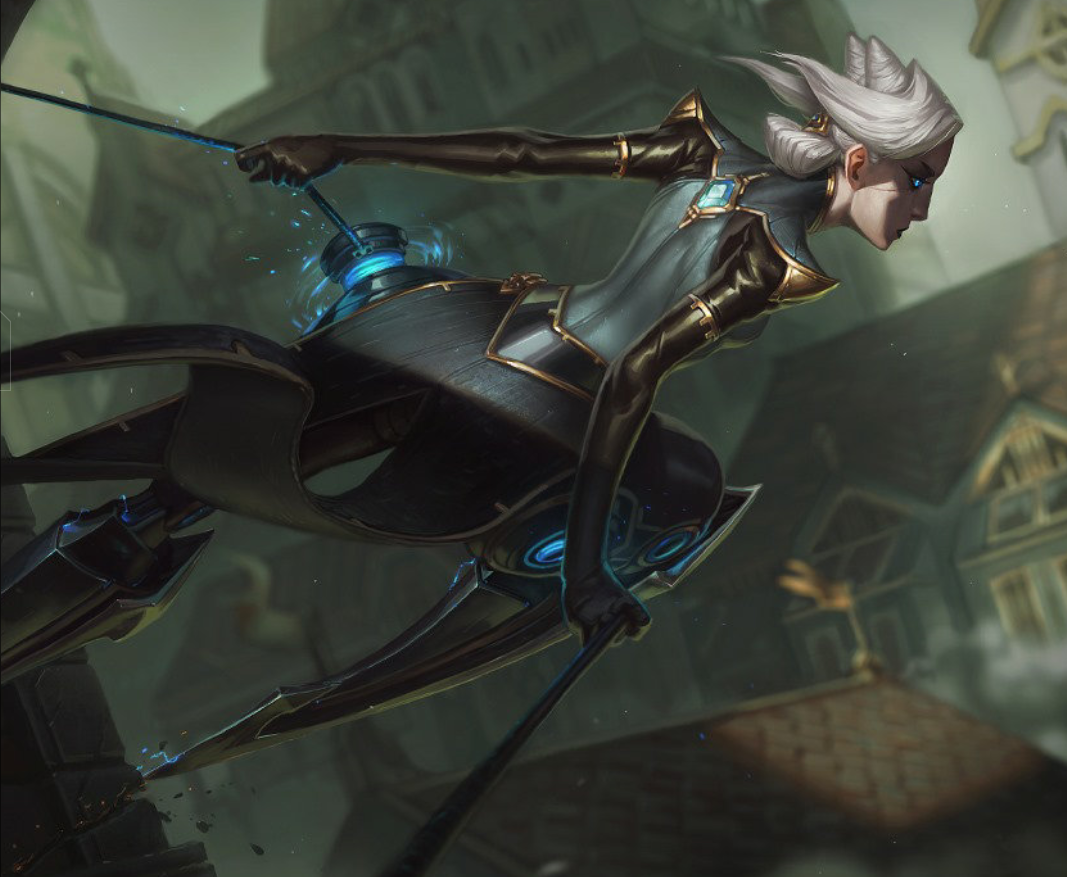
\includegraphics[width=0.9\linewidth]{imagens/camille.png}}
			\caption{Camille}
			\label{fig:camille}
		\end{center}
	\end{figure}
	
	\subsection*{Ornn}
	O Ornn~(Figura \ref{fig:ornn}) de eBorn consegue jogar completamente sem recursos. Sempre que o picka, é campado. Mesmo terminando o jogo 0/28, é ele quem possibilita muitas vezes chegar a vitória com suas ultimates.
	
	\begin{figure}[H]
		\begin{center}
			\boxed{
				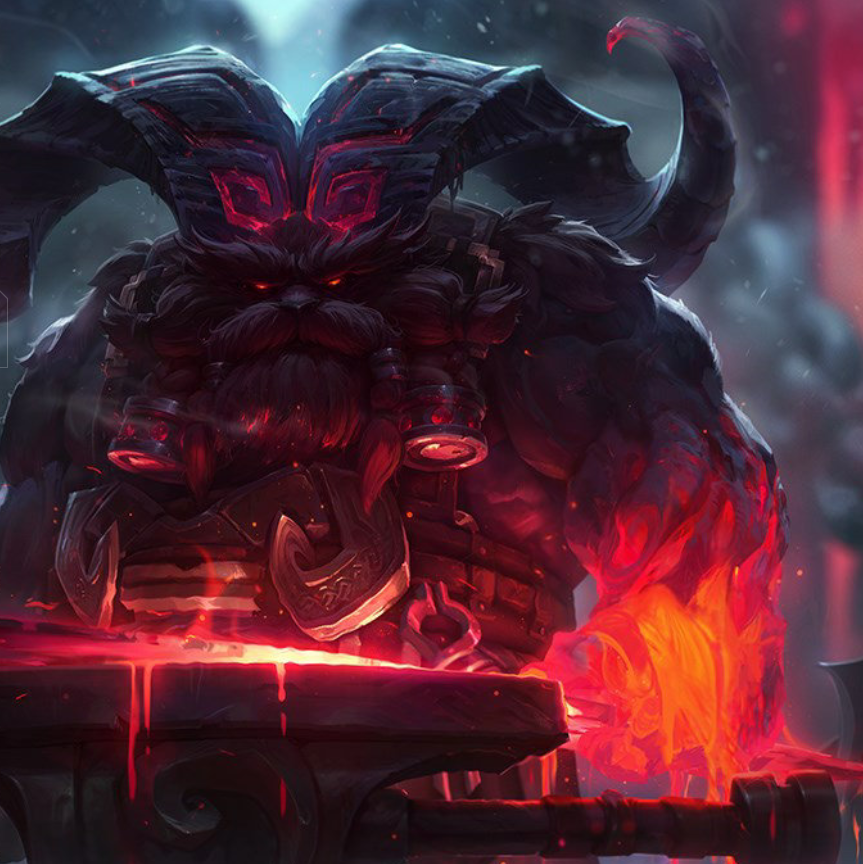
\includegraphics[width=0.9\linewidth]{imagens/ornn.png}}
			\caption{Ornn}
			\label{fig:ornn}
		\end{center}
	\end{figure}
	
	\section*{Premiações}
	\begin{itemize}
		\item 1 Mundial de LoL - 2020
		\item 1 Mid Season Invitational - 2020
		\item 8 Circuitos Brasileiros de League of Legends - Todos os 8 entre 2016 e 2019
		\item 2 League of Legends European Championship - 2020.1, 2020.2
		\item 1 Reality Show Gilette Ult - 2018
	\end{itemize}
	
	\section*{Elos}
	Enquanto no Brasil, eBorn conseguia sempre permanecer entre o  diamante/mestre, porém teve problemas quanto a isso no momento que pisou na Europa, pois lá a dificuldade é maior. Conseguiu apenas chegar no prata.
\end{multicols}    
\newpage

\begin{tabularx}{\linewidth}{@{}m{0.8\textwidth} m{0.2\textwidth}@{}}
	\large{Nome do Jogador: Cleomar Felipe Rabelo Antoszczyszyn} \\
	\large{Posição: Jungler}\\
	\large{Nick: CleoMatador}
\end{tabularx}

\begin{multicols}{2}
	\section*{Sobre o jogador}
	CleoMatador, ao contrário do restante da equipe, começou jogando Mobile Legends, outro jogo MOBA, mas para smartphones. Entretanto, antes mesmo de se tornar profissional no jogo, CleoMatador foi chamados por olheiros da Fnatic (time europeu, uma vez que SlayerCleo é polonês) para realizar um teste na equipe, o que garantiu a vaga ao garoto de 15 anos no time academy da Fnatic. Atuando como jungler, CleoMatador venceu a liga academy no mesmo ano que foi contratado, 2016, e chamou atenção de times maiores, pois na época era o jogador principal daquele time. 
	
	CleoMatador foi então contratado em 2017 pela T2, onde jogou em conjunto com um de seus parceiros atuais, usT. Lá, levaram 4 títulos juntos apenas em 2017 e tornaram a T2 a maior potência do ocidente. Entretanto, o time se desfez ao final da temporada por brigas entre o CleoMatador e o ADC, que não se davam bem por questões internas não reveladas até hoje. Depois disso, CleoMatador se transferiu para a Coréia do Sul, colecionando passagens pela SKT T1 e pela Damwon Gaming. Em 2020, retornou a T2, consagrando esse time o mais completo e bem jogado da história.
	
	Pode-se afirmar que o jungle é um dos maiores do mundo em sua posição, com experiência em controle de mapa e criação de jogadas de pick-off. Seu Master Yi é sua marca, pois CleoMatador gosta de Carrys que jogam com bastante recurso. Experiência em carregar jogos é com ele.
	
	\section*{Campeões Principais}
	\subsection*{Master Yi}
	O principal campeão de CleoMatador (como o nome já diz), é um assassino feito para acumular recursos e carregar jogos. CleoMatador possui uma winrate de 83,4\% com o campeão, o que mostra sua grande experiência com tal.
	
	\begin{figure}[H]
		\begin{center}
			\boxed{
				\centering
				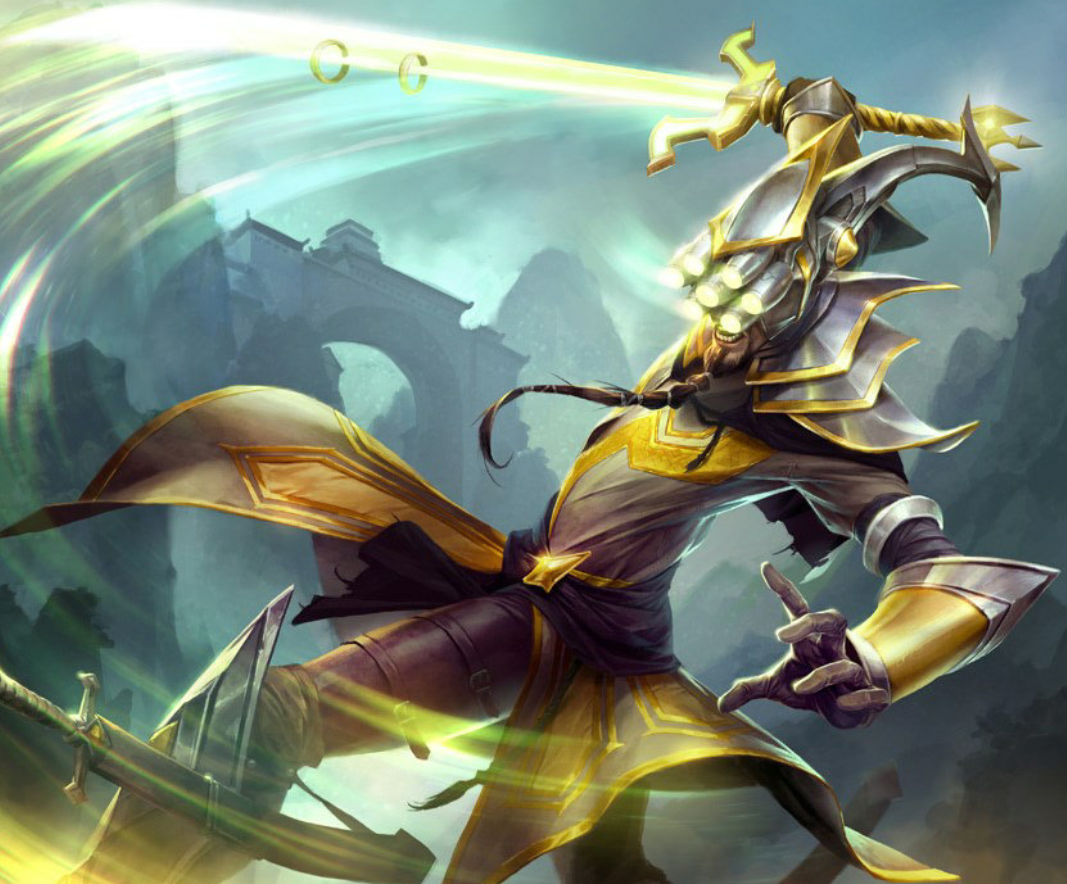
\includegraphics[width=0.9\linewidth]{imagens/yi.png}}
		\end{center}
		\caption{Master Yi}
		\label{fig:fig3}
	\end{figure}
	\subsection*{Olaf}
	Inspirado pela essência viking de seus antepassados, CleoMatador dominou o campeão e hoje atua com ele como ninguém. É o melhor Olaf do mundo, possuindo o "clear" da jungle mais rápido da história.
	
	\begin{figure}[H]
		\begin{center}
			\boxed{
				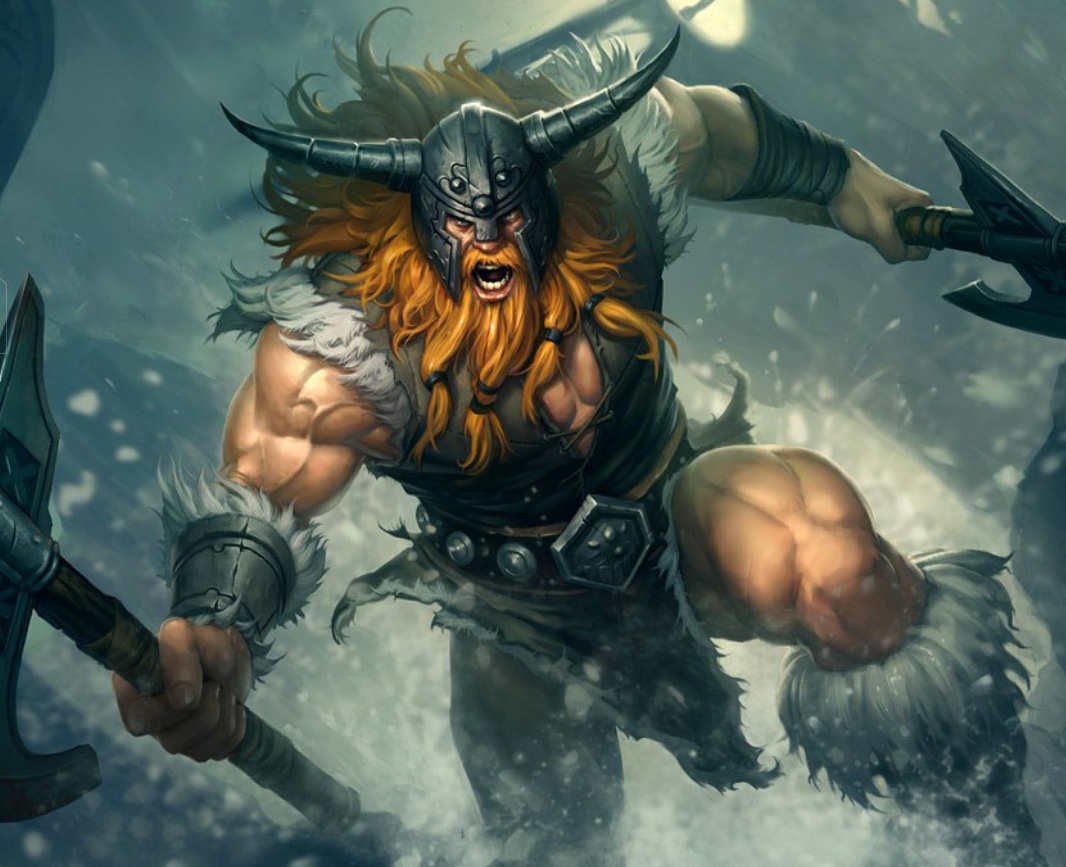
\includegraphics[width=0.9\linewidth]{imagens/olaf.png}}
		\end{center}
		\caption{Olaf}
		\label{fig:fig4}
	\end{figure}
	
	\section*{Premiações}
	\begin{itemize}
		\item 3 Mundiais de League of Legends - 2017, 2018, 2020
		\item 3 Mid Season Invitational - 2017, 2018, 2020
		\item 1 League of Legends European Championship Academy, 2016
		\item 3 League of Legends European Championship, 2017, 2020.1, 2020.2
		\item 4 League of Legends Champions Korea, 2018.1, 2018.2, 2019.1, 2019.2
	\end{itemize}
	
	\section*{Elos}
	Apesar de não dar muita importância para Soloqueue, CleoMatador conquistou o Challenger (elo mais alto do jogo) desde seu primeiro mês no LoL, e de lá nunca mais saiu. Ele nasceu para o jogo!
\end{multicols}

\newpage

\begin{tabularx}{\linewidth}{@{}m{0.8\textwidth} m{0.2\textwidth}@{}}
	\large{Nome do Jogador: Gustavo "Katiau" Ramalho} \\
	\large{Posição: Mid laner}\\
	\large{Nick: usT}
\end{tabularx}

\begin{multicols}{2}
	\section*{Sobre o jogador}  
	UsT é player de League of Legends há 8 anos, e atua profissionalmente há 6. Desde que começou a jogar, se identificou com o League of Legends e construiu uma carreira de sucesso na Mid Lane, tendo domínio completo de campeões do tipo Mage Control e considerável maestria com a classe Assassinos, o que o possibilitou chegar ate onde chegou hoje. É um pilar de suma importância para o time, pois é considerado o player que realiza rotações e concede diversos recursos ao ADCarry, possibilitando que o time cresça e vença as partidas.
	
	Apesar de ter começado a jogar profissionalmente League of Legends apenas há 6 anos, usT é considerado o mentor principal de grandes nomes da Mid Lane do LoL, como Faker, Chovy e Caps. Os 3 jogadores tiveram mentorias particulares que os tornaram os melhores nas posições deles hoje (atrás apenas do próprio usT).
	
	UsT teve participações por apenas 2 times até hoje. Estreando na paiN em 2015, consagrou-se como grande revelação do campeonato brasileiro e foi comprado pela T2, estreando logo como titular e sendo uma das partes fundamentais do time até o final do ano passado, quando se retirou junto a toda equipe.
	
	\section*{Campeões Principais}
	\subsection*{Leblanc}
	A principal campeã de usT, Leblanc~(Figura \ref{fig:leblanc}) é uma maga assassina com uma mecânica consideravelmente difícil de aprender. usT foi eleito, por 7 anos seguidos (até enquanto fora do competitivo), a melhor Leblanc do mundo.
	
	\begin{figure}[H]
		\centering
		\boxed{
			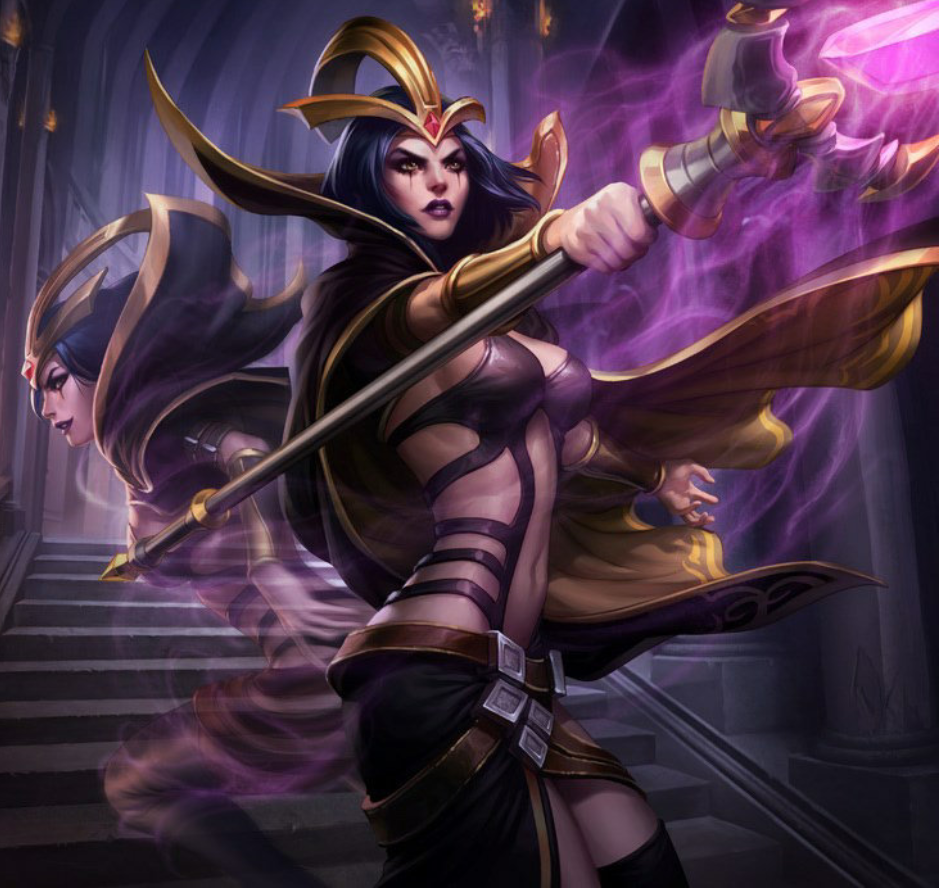
\includegraphics[width=0.9\linewidth]{imagens/leblanc.png}}
		\caption{Leblanc}
		\label{fig:leblanc}
	\end{figure}
	
	\subsection*{Azir}
	usT também domina as mecânicas do Azir, sendo uma ótima opção para jogos que precisam ser levados para o late game. Foi o recordista de farm em uma partida com o campeão, de acordo com o Yodismo, seguindo a filosofia do 100 de farm por minuto.
	
	\begin{figure}[H]
		\centering
		\boxed{
			\includegraphics[width=0.9\linewidth]{imagens/Azir.png}}
		\caption{Azir}
		\label{fig:fig6}
	\end{figure}
	
	\section*{Premiações}
	\begin{itemize}
		\item 2 Mundiais de League of Legends, um em  2017 e outro em 2020
		\item 3 Mid Season Invitational - 2017, 2019, 2020
		\item 1 Circuito Brasileiro de League of Legends - 2015
		\item 6 League of Legends European Championship - 2017.1, 2017.2, 2018.1, 2019.1, 2020.1, 2020.2
	\end{itemize}
	
	\section*{Elos}
	UsT, apesar de todos os seus feitos, não conseguiu pegar elos muito altos na SoloQueue do LoL... De 2015 ate 2017 foi Ouro, conquistando o platina em 2018. Pelo menos em 2020, numa ótima fase de sua carreira, chegou ao diamante\cite{kou}.
	\begin{figure}[H]
		\centering
		\boxed{
			
\includegraphics[width=0.6\linewidth]{imagens/diamante4.jpeg}}
		\caption{usT no High Elo }
		\label{fig:elos}
	\end{figure}
\end{multicols}

\begin{tabularx}{\linewidth}{@{}m{0.8\textwidth} m{0.2\textwidth}@{}}
	\large{Nome do Jogador: João Victor Mendes} \\
	\large{Posição: ADCarry}\\
	\large{Nick: jaodasnevi}
\end{tabularx}

\begin{multicols}{2}
	\section*{Sobre o jogador}
	Jaodasnevi nasceu em Wuhan, na China, de uma família alemã que vivia na região .Desde pequeno teve muita afinidade com armas porque treinava tiro-ao-alvo com seu pai, e, quando começou a jogar LoL (em 2015), não pensou em jogar em outra posição que nao fosse ADC (atirador). jaodasnevi se mostrou como uma grande promessa do cenário chinês com apenas 2 jogos no LoL, e foi contratado pela Edward Gaming em 2016, onde estreou a dupla de Bot mais proativa do cenário de LoL Mundial, jaodasnevi e antarcticite. Desde então, a dupla foi inseperável no jogo e perderam apenas 1 split na China, no final de 2019 quando jaodasnevi e antarcticite tiveram um desentendimento e se separaram.
	
	Em 2020, fizeram as pazes e foram para a Europa onde, em conjunto com CleoMatador, eBorn e usT criaram o maior exódia do LoL mundial. Inclusive, vale ressaltar que jaodasnevi foi considerado o MVP desse time em 2020 por diversas revistas francesas.
	
	Até o dia de reunir o Exódia, jaodasnevi já tinha treinado diversos outros ADC's mundiais, sendo mestre de Uzi, Jackeylove e recentemente, do Viper. É um ADC COMPLETO. Pode-se dizer que jaodasnevi domina todo tipo de ADC, dos Carrys aos mais utilitys. Seu principal campeão é o Aphelios (pois lembra um pouco de sua personalidade emo), mas também domina outros como Xayah e Caitlyn.
	
	\section*{Campeões Principais}
	\subsection*{Aphelios}
	O campeão que jaodasnevi mais tem dominância, é um atirador que carrega 4 tipos de armas poderosas. Não há Aphelios no mundo melhor que o dele!!
	
	\begin{figure}[H]
		\centering
		\boxed{
			
\includegraphics[width=0.9\linewidth]{imagens/aphelios.png}}
		\caption{Melhor Aphelios do mundo}
		\label{fig:fig7}
	\end{figure}
	
	\subsection*{Xayah}
	Sua Xayah é uma ótima dupla para o Rakan de Alic, pois os campeões nasceram para serem jogados juntos. É um expert com esse time de ADC.
	\begin{figure}[H]
		\centering
		\boxed{
			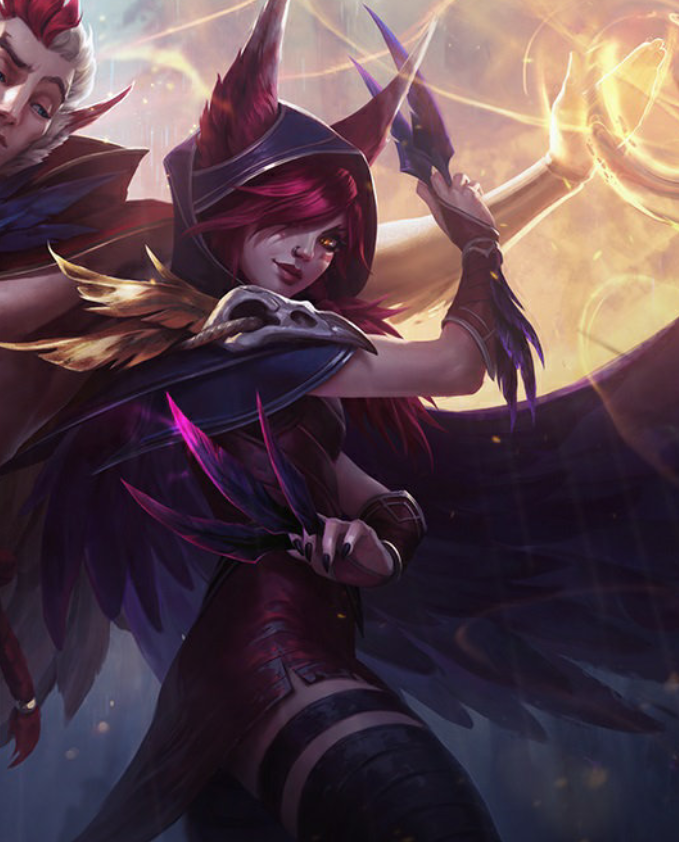
\includegraphics[width=0.9\linewidth]{imagens/xayah.png}}
		\caption{Xayah}
		\label{fig:fig8}
	\end{figure}
	
	\section*{Prêmiações}
	\begin{itemize}
		\item 2 Mundiais de League of Legends - 2016, 2020
		\item 7 League of Legends Pro League( LPL - China) - 2016.1, 2016.2, 2017.1, 2017.2, 2018.1, 2018.2, 2019.1
		\item 2 Mid Season Invitational - 2016, 2020
		\item 2 League of Legends European Championship - 2020.1, 2020.2
	\end{itemize}
	
	\section*{Elos}
	Jaodasnevi conseguiu pegar Challenger com 2 jogos no LoL, feito que ninguem até hoje conseguiu compreender. Pela dinâmica e lógica do jogo, isso seria algo impossível, mas até a própria Riot Games considerou o jogador como "extremamente incomum", o que, segundo a empresa, era motivo suficiente para tal feitio.
	
\end{multicols}

\newpage

\begin{tabularx}{\linewidth}{@{}m{0.8\textwidth} m{0.2\textwidth}@{}}
	\large{Nome do Jogador: Alice Pereira de Aguilar Penido} \\
	\large{Posição: Support}\\
	\large{Nick: antarcticite}
\end{tabularx}

\begin{multicols}{2}
	\section*{Sobre a jogadora}
	Antarcticite vem de uma família rica de brasileiros que moram no Japão que sempre a incentivou a estudar para construir um ótimo futuro. Entretanto, foi nos jogos que antarcticite encontrou um caminho para a felicidade, e, assim, conseguiu pegar emprestado 100 mil do pai para viver seu sonho na China (melhor região de LoL) de atingir o nível profissional. Começou em 2012 mas conseguiu chegar em alto patamar em 2016, quando fez dupla de bot com jaodasnevi, que os tornou os melhores em suas posições. De lá pra cá, conquistou diversos títulos da LPL, chegando a um desentendimento com jaodasnevi em 2019 que o fizeram se separar. Ainda assim, voltaram a jogar juntos em 2020 pela T2.
	
	Antarcticite é uma suporte que compreende perfeitamente rotações de mapa, patching da Jungle para fazer boas rotações com CleoMatador e uma legítima entendedora de builds\cite{kou2}. Foi, a propósito, a treinadora de Mata e de BeryL, suportes extremamentes consagrados em suas posições. 
	
	Domina campeões suportes tanks e de utility, e o seu principal é o Rakan. Também possui experiência com a Morgana, pois domina a ideia de skillshot como ninguém.
	
	\section*{Campeões Principais}
	\subsection*{Rakan}
	Seu principal campeão, Rakan, é ótimo para teamfights e controle de grupo, além de possibilitar antarcticite uma movimentação no mapa excelente!!
	\begin{figure}[H]
		\centering
		\boxed{
			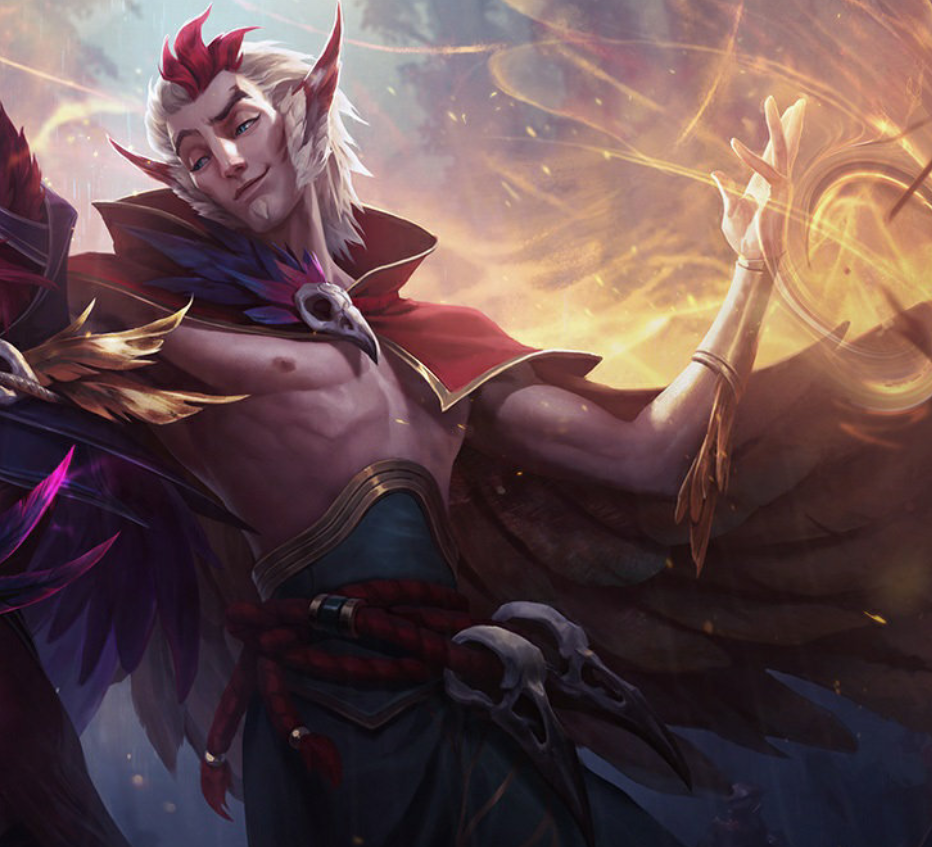
\includegraphics[width=0.9\linewidth]{imagens/rakan.png}}
		\caption{Rakan}
		\label{fig:fig9}
	\end{figure}
	
	\subsection*{Morgana}
	Antarcticite domina Morgana como ninguém, mesmo que a campeão não apareça muito no meta do competitivo. Mesmo com esse entrave, a Morgana da jogadora é sempre muito decisiva!
	\begin{figure}[H]
		\centering
		\boxed{
			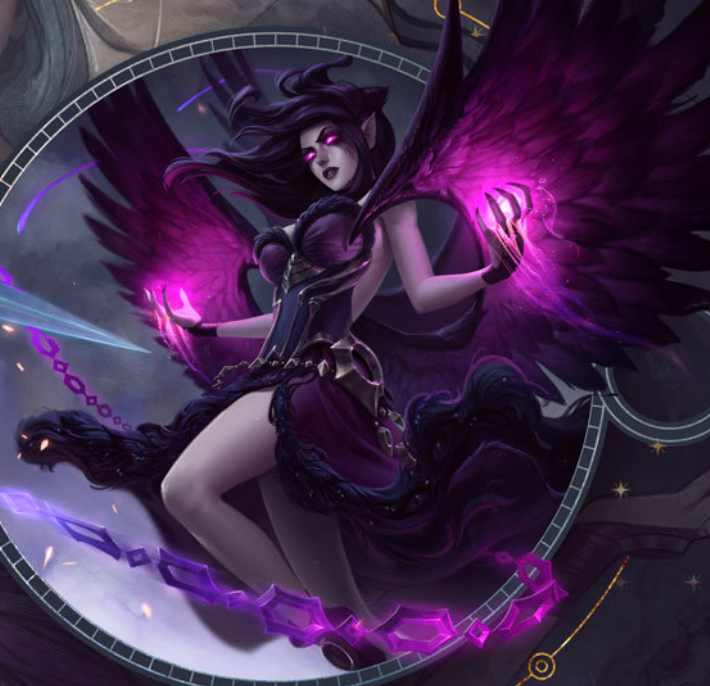
\includegraphics[width=0.9\linewidth]{imagens/morgana.png}}
		\caption{Morgana}
		\label{fig:fig10}
	\end{figure}
	
	\section*{Premiações}
	\begin{itemize}
		\item 2 Mundiais de League of Legends - 2016, 2020
		\item 7 League of Legends Pro League(LPL - China) - 2016.1, 2016.2, 2017.1, 2017.2, 2018.1, 2018.2, 2019.1
		\item 2 Mid Season Invitational - 2016, 2020
		\item 2 League of Legends European Championship - 2020.1, 2020.2
	\end{itemize}
	
	\section*{Elos}
	Com diversos treinamentos, antarcticite conseguiu pegar Mestre em 2015 e Challenger em 2016, mas até essa época tinha conseguido apenas ficar no platina. Depois daí, nunca mais saiu do High Elo e sempre se mostrou como uma suporte de ponta, chegando a ser considerada por muitos a melhor do mundo.
\end{multicols}

		
		\bibliographystyle{acm}
		\bibliography{referencias/referencias.bib}
	}
\end{document}